\documentclass[english, 12pt, a4paper, sci, utf8, a-2b, online]{aaltothesis}

%% DO NOT MOVE OR REMOVE \setupthesisfonts
\setupthesisfonts

%% Add here the packges you need
\usepackage{graphicx}


%% For tables that span multiple pages; used to split a paraphrasing example in
%% the appendix. If you don't need it, remove it.
\usepackage{longtable}

%% A package for generating Creative Commons copyright terms. If you don't use
%% the CC copyright terms, remove it, since otherwise undesired information may
%% be added to this document's metadata.
\usepackage[type={CC}, modifier={by-nc-sa}, version={4.0}]{doclicense}
%% Find below three examples for typesetting the CC license notice.


%% Edit to conform to your degree programme
%% Capitalise the words in the name of the degree programme: it's a name
\degreeprogram{Computer, Communication and Information Sciences}
\major{Macadamia}
% \major{Machine Learning, Data Science and Artificial Intelligence}
\univdegree{MSc}
\thesisauthor{Stefan Rua}

%% Your thesis title and possible subtitle comes here and possibly, again,
%% together with the Finnish or Swedish abstract. Do not hyphenate the title
%% (and subtitle), and avoid writing too long a title. Should LaTeX typeset a
%% long title (and/or subtitle) unsatisfactorily, you might have to force a
%% linebreak using the \\ control characters. In this case...
%% * Remember, the title should not be hyphenated!
%% * A possible 'and' in the title should not be the last word in the line; it
%%   begins the next line.
%% * Specify the title (and/or subtitle) again without the linebreak characters
%%   in the optional argument in box brackets. This is done because the title
%%   is part of the metadata in the pdf/a file, and the metadata cannot contain
%%   linebreaks.
\thesistitle{SAM2 pseudolabeling for instance segmentation}
\place{Espoo}
%% The date for the bachelor's thesis is the day it is presented
\date{30 September 2025}

%% Thesis supervisor
%% Note the "\" character in the title after the period and before the space
%% and the following character string.
%% This is because the period is not the end of a sentence after which a
%% slightly longer space follows, but what is desired is a regular interword
%% space.
\supervisor{Jorma Laaksonen}

%% Advisor(s)---two at the most---of the thesis. Check with your supervisor how
%% many official advisors you can have.
\advisor{Julius Pesonen (MSc)}

%% If you do your thesis work in a company of other institute, give the name of
%% the company or instution here. Otherwise, leave the macro empty, comment it
%% out, or remove it. This will remove this field from the abstract page.
\collaborativepartner{Finnish Geospatial Research Institute FGI}

%% Aaltologo: syntax:
%% \uselogo{?|!|''}
%% The logo language is set to be the same as the thesis language.
%%
\uselogo{?}
%\uselogo{!}
%\uselogo{''}
%%

%%%%%%%%%%%%%%%%%%               COPYRIGHT TEXT               %%%%%%%%%%%%%%%%%%
%%%%%%%%%%%%%%%%%%%%%%%%%%%%%%%%%%%%%%%%%%%%%%%%%%%%%%%%%%%%%%%%%%%%%%%%%%%%%%%%

%% Copyright of a work is with the creator/author of the work regardless of
%% whether the copyright mark is explicitly in the work or not. You may, if you
%% wish---we encourage you to do so---publish your work under a Creative
%% Commons license (see creativecommons.org), in which case the license text
%% must be visible in the work. Write here the copyright text you want using the
%% macro \copyrighttext, which writes the text into the metadata of the pdf file
%% as well.
%%
%% Syntax:
%% \copyrigthtext{metadata text}{text visible on the page}
%%
%% CHOOSE ONE OF THE COPYRIGHT NOTICE STYLES BELOW.
%% IF USING THE CC TERMS, CHOOSE THE LICENSE YOU WANT TO USE.
%% The different CC licenses are listed at 
%% https://creativecommons.org/about/cclicenses/.
%% If you use the icons from the dolicense.sty package, add the package above
%% (\usepackage{dolicense}).
%% IMPORTANT NOTE!! Manually write the CC text in the \copyrighttext metadata
%% text field.
%%
%% NOTE: In the macros below, the text written in the metadata must have a
%% \noexpand macro before the \copyright special character. When not in pdf/a
%% mode (i.e. a-1b or a-2b are not specified in \documentclass), two \noexpands
%% are required in the metadata text to correctly render the copyright mark in
%% the pdf metadata. In pdf/a mode one \noexpand suffices.
%%
%% EXAMPLE OF PLAIN COPYRIGHT TEXT
%% The macros \copyright and \year below must be separated by the \ character 
%% (space chacter) from the text that follows. The macros in the argument of the
%% \copyrighttext macro automatically insert the year and the author's name.
%% (Note! \ThesisAuthor is an internal macro of the aaltothesis.cls class file).
%%
%\copyrighttext{Copyright \noexpand\textcopyright\ \number\year\ \ThesisAuthor}
%{Copyright \textcopyright{} \number\year{} \ThesisAuthor}
%%
%% Of course, the same text could have simply been written as
%% \copyrighttext{Copyright \noexpand\copyright\ 2018 Eddie Engineer}
%% {Copyright \copyright{} 2022 Eddie Engineer}
%%
%% EXAMPLES OF CC LICENSE: different ways to display the same license
%% 1. A simple Creative Commons license text with a link to the copyright notice:
%\copyrighttext{\noexpand\textcopyright\ \number\year. This work is 
%	licensed under a CC BY-NC-SA 4.0 license.}{\textcopyright{} 
%	\number\year. This work is licensed under a 
%	\href{https://creativecommons.org/licenses/by-nc-nd/4.0/}{CC BY-NC-SA 4.0} 
%	license.}
%
%% To get the URL of the license of your choice, go to 
%% https://creativecommons.org/about/cclicenses/, click on the chosen license
%% you want to use, and copy-and-paste the URL in the macro \href above.
%%
%% 2. A short Creative Commons license text containing the respective CC icons
%% (requires the package dolicense.sty to be added in the preamble as done
%% above) and a link to the corresponding Creative Commons license webpage (see
%% the dolicense package documentation for other license icons):
%\copyrighttext{\noexpand\textcopyright\ \number\year. This work is licensed
%	under a CC BY-NC-SA 4.0 license.}{
%	\parbox{95mm}{\noindent\textcopyright\ \number\year. \doclicenseText} 
%	\hspace{1em}\parbox{35mm}{\doclicenseImage}
%}
%%
%% 3. An expanded Creative Commons license text containing the respective CC
%% icons text and as generated by the dolicense.sty package (the license is set
%% via package options in \usepackage[options]{dolicense} above; see the
%% dolicense package documentation for other license texts and icons):
\copyrighttext{\noexpand\textcopyright\ \number\year. This work is 
	licensed under a Creative Commons "Attribution-NonCommercial-ShareAlike 4.0 
	International" (BY-NC-SA 4.0) license.}{\noindent\textcopyright\ \number
	\year \ \doclicenseThis}
%%%%%%%%%%%%%%%%%%%%%%%%%%%%%%%%%%%%%%%%%%%%%%%%%%%%%%%%%%%%%%%%%%%%%%%%%%%%%%%%


%% The English abstract:
%% All the details (name, title, etc.) on the abstract page appear as specified
%% above.
%% Thesis keywords:
%% Note! The keywords are separated using the \spc macro
\keywords{pseudolabeling\spc instance segmentation\spc forestry}

%% The abstract text. This text in one paragraph is included in the metadata of
%% the pdf file as well as the abstract page. To have paragraphs in your
%% abstract rewrite it in the abstarct environment as described below.
\thesisabstract{
    Yappidi-yap, lorem ipsum etc.
}

%% You can prevent LaTeX from writing into the xmpdata file (it contains all the 
%% metadata to be written into the pdf file) by setting the writexmpdata switch
%% to 'false'. This allows you to write the metadata in the correct format
%% directly into the file thesistemplate.xmpdata.
%\setboolean{writexmpdatafile}{false}


%% All that is printed on paper starts here
%%
\begin{document}

%% Create the coverpage
%%
\makecoverpage

%% Typeset the copyright text.
%% If you wish, you may leave out the copyright text from the human-readable
%% page of the pdf file. This may seem like a attractive idea for the printed
%% document especially if "Copyright (c) yyyy Eddie Engineer" is the only text
%% on the page. However, the recommendation is to print this copyright text.
%%
\makecopyrightpage

\clearpage
%% Note that when writing your thesis in English, place the English abstract
%% first followed by the possible Finnish or Swedish abstract.

%% Abstract text
%% All the details (name, title, etc.) on the abstract page appear as specified
%% above. Add your abstarct text with paragraphs here to have paragraphs in the
%% visible abstract page. Nonetheless, write the abstarct text without
%% paragraphs in the macro \thesismacro so that it is added to the metadata as
%% well.
%%
\begin{abstractpage}[english]
    Yappidi-yap, lorem ipsum etc.
\end{abstractpage}

%% The text in the \thesisabstract macro is stored in the macro \abstractext, so
%% you can use the text metadata abstract directly as follows:
%%
%\begin{abstractpage}[english]
%	\abstracttext{}
%\end{abstractpage}

%% Force a new page so that the possible Finnish or Swedish abstract does not
%% begin on the same page
%%
\newpage
%%
%% Abstract in Finnish. Delete if you don't need it. 
%%
%% Respecify those fields that differ from the earlier specification or simply
%% respecify all fields.
\thesistitle{SAM2 pseudolabelöinti instanssisegmentaatiokoulutuksessa}
% \thesissubtitle{Opinnäytteen mahdollinen alaotsikko}
\supervisor{Jorma Laaksonen}
\advisor{DI Julius Pesonen}
\degreeprogram{Computer, Communication and Information Sciences}
\major{Macadamia}
\collaborativepartner{Paikkatietokeskus FGI}
\date{30.9.2025}
%% The keywords need not be separated by \spc now.
\keywords{pseudolabelöinti, instanssisegmentaatio, metsäily}
%% Abstract text
\begin{abstractpage}[finnish]
    Höpötihöp, lorem ipsum jne.
\end{abstractpage}

\dothesispagenumbering{}

%% Table of contents. 
%%
\thesistableofcontents

%% \clearpage is similar to \newpage, but it also flushes the floats (figures
%% and tables).
%%
\cleardoublepage

%% Text body begins. Note that since the text body is mostly in Finnish the
%% majority of comments are also in Finnish after this point. There is no point
%% in explaining Finnish-language specific thesis conventions in English.
%% This text will be translated to English soon.
%%
\section{Introduction}
\label{sec:intro}

%% Leave page number of the first page empty
%% 
\thispagestyle{empty}

Airborne remote sensing based tree mapping methods are used for forest health monitoring \cite{ecke} and city planning \cite{velasquez} due to their efficiency, but the training process is often bottlenecked by creating high quality annotations manually. 
The goal of this study is to test if training results can be improved in instance segmentation tasks by refining coarse segments calculated from a canopy height model (CHM) using Segment Anything Model 2 (SAM2) \cite{sam2}.

\newpage
\section{Related Work}

The previous version of SAM2, SAM has been assessed for tree crown instance segmentation on drone imagery \cite{sam-treecrown}. The study uses SAM in the following ways: generating masks without any prompts, generating masks with digital surface model (DSM) maxima as point prompts, and prompting SAM with predictions from a trained Mask R-CNN model. Of these, the last approach is closest to the one examined here.

Another study examining SAM for remote sensing use proposes RSPrompter \cite{rsprompter}, a method that learns to generate prompts from the SAM's image encoder, then feeding them to the decoder.

\newpage
\section{Materials and Methods}

\subsection{Datasets}

The main dataset consists of a multispectral orthophoto spanning approximately 2 km$^2$ and CHM-based coarse tree crown segments. The orthophoto covers both forest and urban area, has a GSD of 2.5 cm, and contains blue, green, red, near-infrared, ???, and thermal bands.

- taken by drone/helicopter?

\subsection{Models}

SAM2 is used for the pseudolabeling task and Mask R-CNN \cite{maskrcnn} for the supervised instance segmentation.

\subsection{Methods}

First the coarse segments were pseudolabeled using SAM2, indexing the orthphoto in a grid with a window of size 1024 and a stride of 512. For each window, only the segments whose centroids were located in the central 512x512 square of the window were selected for pseudolabeling. Then, the bounding box of each segment was passed as a prompt to SAM2, and the largest connected component of the output mask was saved as the pseudolabel. These parameters for the window size and stride were selected in order to avoid stitching artifacts and to provide SAM2 with images mathcing the native input resolution of the model.

A small test area of 25 trees was segmented manually. To evaluate the quality of the coarse segments and quantify the effect of SAM2 pseudolabeling, the coarse segments and pseudolabels were compared to the manual segments using the Jaccard index \cite{jaccard}:

$$
J(A, B) = \frac{|A \cap B|}{|A \cup B |},
$$

where A and B are the segments to be compared. Then, a Mask R-CNN model with a ResNet-50 \cite{resnet} backbone was trained separately on both the coarse segments and pseudolabels.

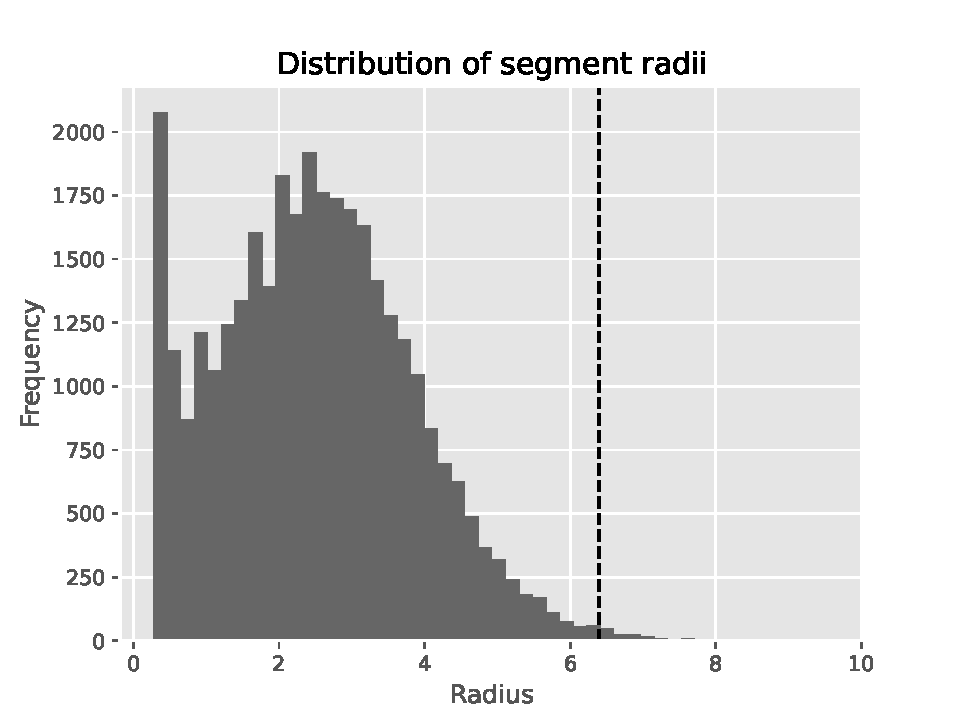
\includegraphics{figures/radii.pdf}

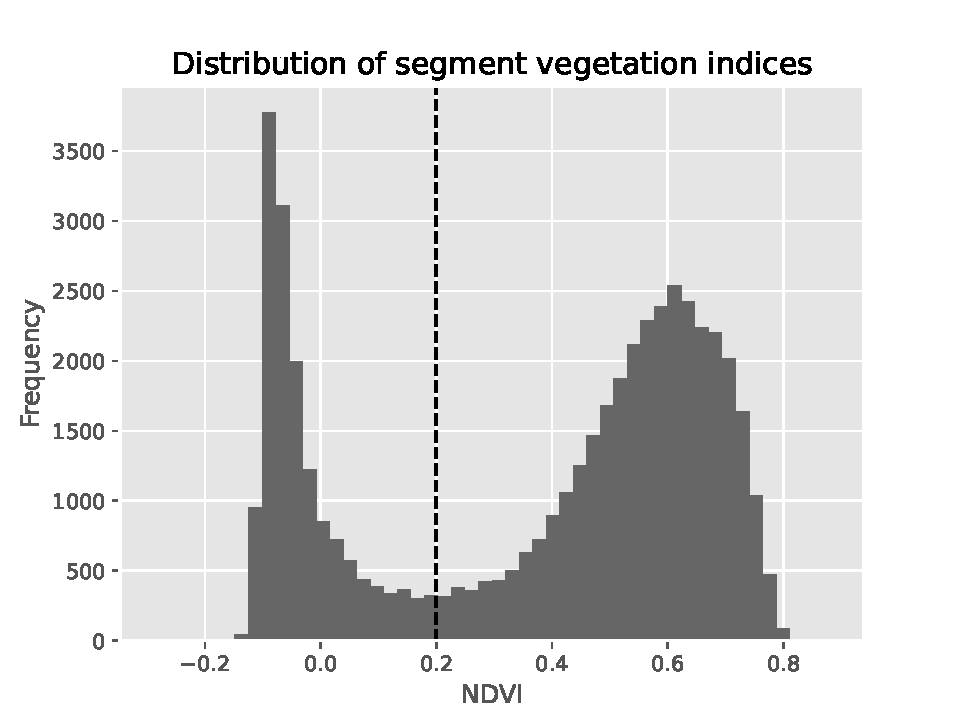
\includegraphics{figures/ndvi.pdf}

\section{Results}

\section{Discussion}

\section{Conclusions}

\clearpage

\thesisbibliography
\bibliographystyle{IEEEtran}
\bibliography{references}

\end{document}
